\documentclass[11pt]{article}

\usepackage[margin=1in]{geometry}
\usepackage{amsmath, amssymb, amsthm, bm}
\usepackage{booktabs}
\usepackage{graphicx}
\usepackage{multirow}
\usepackage{hyperref}
\usepackage{enumitem}
\usepackage{xcolor}
\usepackage{natbib}
\usepackage{setspace}
\usepackage{caption}
\usepackage{subcaption}

\usepackage{listings}
\usepackage{xcolor}  % for syntax highlighting
\usepackage{amsmath} % for equations in Appendix E
\usepackage{amssymb}
\hypersetup{
  colorlinks=true,
  linkcolor=blue,
  citecolor=blue,
  urlcolor=blue
}

\setlength{\parskip}{0.45em}
\setlength{\parindent}{0pt}
\setstretch{1.03}

\title{\textbf{Is International Football Becoming More Random?}\\
A Bayesian Analysis of Competitive Balance Over Time}
\author{
Blasius Halley Theo Boniarga \and
Helmi Hidayat Rouf \and
Louis Charistias Saragih
}
\date{April 19, 2026}

\begin{document}
\maketitle

\textbf{Repository:} \url{https://github.com/HelmiHRouf/bayesian-worldcup-prediction}

\textbf{Contributions.} 
Blasius Halley Theo Boniarga focused on data collection and preprocessing.
Helmi Hidayat Rouf focused on hierarchical model specification and Stan implementation.
Louis Charistias Saragih focused on posterior computation, model comparison, and report drafting.
All team members contributed to interpretation, figure design, and final editing.

\section{Introduction}

International football is often described as increasingly unpredictable: established powers still matter, but upsets seem more common than in earlier decades.
This project studies that claim using a Bayesian perspective.
Our guiding question is:
\begin{quote}
\emph{Has international football become more random over time?}
\end{quote}

To answer this, we interpret ``more random'' as \emph{greater parity}: if national teams are closer in latent strength, match outcomes should be harder to predict.
Using historical international match data, we estimate how the cross-team dispersion of latent strengths changes over time.
A downward trend in dispersion is interpreted as evidence of increasing competitive balance and thus greater randomness.

Our project is designed to satisfy the core course requirements.
We analyze a real dataset, describe two Bayesian models, and compare at least two posterior approximation methods.
We also include model criticism and discussion of numerical stability, especially for the more ambitious dynamic model.

\section{Data and Related Work}

\subsection{Dataset}

Our main dataset is the \emph{International Football Results (1872--present)} dataset, containing match dates, teams, and scores for men's international football.
The project repository also identifies FIFA rankings as a potential auxiliary dataset, though the analysis in this report uses match outcomes as the primary source of information.
After preprocessing, each match contributes:
\[
(\text{home team},\ \text{away team},\ \text{home goals},\ \text{away goals},\ \text{time index}).
\]

The long time span is both the main strength and the main challenge of the dataset.
It allows us to study historical trends in competitive balance, but it also introduces substantial nonstationarity: rule changes, globalization, tactical evolution, and varying data quality across decades.

\subsection{Literature Context}

Statistical modelling of football scores is commonly based on Poisson models with latent attack and defense effects, as in Dixon and Coles (1997). A Bayesian hierarchical formulation is given by Baio and Blangiardo (2010), who model team strengths and perform inference using WinBUGS. These approaches are primarily designed for match prediction and typically assume team strengths are static within a given period.

Our work builds on this framework but focuses on the evolution of competitive balance over time. Rather than predicting individual match outcomes, we study how the distribution of latent team strengths changes across years, using a long historical dataset. In particular, Model 2 introduces a time-varying structure in which the dispersion parameter evolves dynamically, allowing us to capture long-run trends in parity. We also implement the model in Stan using Hamiltonian Monte Carlo and compare it with variational inference, providing a modern Bayesian workflow with explicit uncertainty quantification for competitive balance.

\section{Bayesian Formulation}

\subsection{Interpretation of Randomness}

We do not model ``randomness'' as an ad hoc noise parameter.
Instead, we define it through latent competitive balance.
If team strengths in a given era or year are highly dispersed, strong teams and weak teams are easier to distinguish, making results more predictable.
If strengths are tightly clustered, outcomes become harder to anticipate.
Therefore, the key object of interest is the spread parameter
\[
\sigma,
\]
or its time-varying analogue \(\sigma_y\), governing the variation of team strengths.

\subsection{Model 1: Era-Based Competitive Balance}

Let \(i=1,\dots,N\) index matches, \(t=1,\dots,T\) teams, and \(e=1,\dots,E\) eras. Let \(h(i)\) and \(a(i)\) denote the home and away teams in match \(i\), and let \(e(t)\) denote the era of team \(t\).

\paragraph{Likelihood.}
\begin{align}
y_i^{(H)} &\sim \mathrm{Poisson}\!\left(\lambda_i^{(H)}\right), &
\log \lambda_i^{(H)} &= \mu + \alpha_{h(i)} - \beta_{a(i)}, \\
y_i^{(A)} &\sim \mathrm{Poisson}\!\left(\lambda_i^{(A)}\right), &
\log \lambda_i^{(A)} &= \mu + \alpha_{a(i)} - \beta_{h(i)}.
\end{align}

\paragraph{Hierarchical effects.}
\begin{align}
\alpha_t &\sim \mathcal{N}\!\left(0,\sigma_{\alpha,e(t)}^2\right), \\
\beta_t  &\sim \mathcal{N}\!\left(0,\sigma_{\beta,e(t)}^2\right).
\end{align}

\paragraph{Priors.}
\begin{align}
\mu &\sim \mathcal{N}(0,1), \\
\sigma_{\alpha,e} &\sim \mathcal{N}(0,1)\,\mathbf{1}\!\left\{\sigma_{\alpha,e}\ge 10^{-3}\right\}, \\
\sigma_{\beta,e}  &\sim \mathcal{N}(0,1)\,\mathbf{1}\!\left\{\sigma_{\beta,e}\ge 10^{-3}\right\}.
\end{align}

\paragraph{Posterior and quantity of interest.}
\[
p\!\left(\mu,\alpha,\beta,\sigma_\alpha,\sigma_\beta \mid y\right),
\qquad
\left\{\sigma_{\alpha,e},\sigma_{\beta,e}\right\}_{e=1}^E.
\]
Smaller \(\sigma_{\alpha,e}\) and \(\sigma_{\beta,e}\) indicate greater parity.

\subsection{Model 2: Time-Varying Competitive Balance}

Let \(y=1,\dots,Y\) index years, and let \(y(i)\) denote the year of match \(i\).

\paragraph{Likelihood.}
\begin{align}
y_i^{(H)} &\sim \mathrm{Poisson}\!\left(\lambda_i^{(H)}\right), &
\log \lambda_i^{(H)} &= \mu + \alpha_{h(i),y(i)} - \beta_{a(i),y(i)}, \\
y_i^{(A)} &\sim \mathrm{Poisson}\!\left(\lambda_i^{(A)}\right), &
\log \lambda_i^{(A)} &= \mu + \alpha_{a(i),y(i)} - \beta_{h(i),y(i)}.
\end{align}

\paragraph{Team-year effects.}
\begin{align}
\alpha_{t,y} &\sim \mathcal{N}\!\left(0,\sigma_y^2\right), \\
\beta_{t,y}  &\sim \mathcal{N}\!\left(0,\sigma_y^2\right).
\end{align}

\paragraph{Dynamic dispersion.}
\begin{align}
\log \sigma_y &= \log \sigma_{y-1} + \varepsilon_y, \qquad y=2,\dots,Y, \\
\varepsilon_y &\sim \mathcal{N}\!\left(0,\omega^2\right).
\end{align}

\paragraph{Priors.}
\begin{align}
\mu &\sim \mathcal{N}(0,1), \\
\sigma_1 &\sim \mathrm{Half\text{-}Normal}(0,1), \\
\omega &\sim \mathrm{Half\text{-}Normal}(0,0.5).
\end{align}

\paragraph{Posterior and quantity of interest.}
\[
p\!\left(\mu,\alpha,\beta,\sigma,\omega \mid y\right),
\qquad
\left\{\sigma_y\right\}_{y=1}^Y.
\]
Smaller \(\sigma_y\) indicates greater parity over time.

\paragraph{Implementation.}
The MH implementation targets the marginalized posterior
\[
p\!\left(\mu,\sigma,\omega \mid y\right),
\]
while the Stan implementation samples the full model using a non-centered parameterization.

\section{Posterior Computation}

A project requirement is to compare at least two posterior approximation methods.
We therefore used both HMC/NUTS and variational inference.

\subsection{Metropolis-Hastings}
As a baseline inference method, we implemented a custom Metropolis-Hastings sampler
in R for both models. Because directly sampling the full joint posterior over all
team-year strength parameters is computationally intractable in plain R, we
marginalized out the team-level attack and defense strengths analytically.
Since these are Normal random effects, their marginal contribution to the likelihood
can be approximated via Monte Carlo integration, leaving a lower-dimensional
posterior over only the key quantities of interest.

For Model 1, the MH sampler targets the posterior over $\mu$,
$\{\sigma_{\alpha,e}\}_{e=1}^{7}$, and $\{\sigma_{\beta,e}\}_{e=1}^{7}$ ---
the baseline log-rate and the era-level attacking and defensive strength dispersions.
We used a block updating scheme, proposing each parameter individually to avoid
the collapse in acceptance probability that occurs with high-dimensional joint proposals.
Likelihood contributions were cached per era so that updating $\sigma_{\alpha,e}$
or $\sigma_{\beta,e}$ for a single era only requires recomputing that era's likelihood,
not the full dataset.

For Model 2, the MH sampler targets the posterior over $\mu$, $\omega$, and
$\{\log \sigma_y\}_{y=1}^{Y}$ --- the baseline rate, the random walk volatility,
and the full trajectory of year-level team strength dispersion.
The same block updating scheme was applied, with each $\log \sigma_y$ updated
individually. An incremental prior difference calculation was used so that
updating $\log \sigma_y$ only recomputes the at most three affected terms in
the random walk prior rather than the full prior sum.


\subsection{HMC/NUTS}

For both models, posterior sampling in Stan via \texttt{sample()} uses HMC with the No-U-Turn Sampler (NUTS).
This method is asymptotically exact and serves as the main reference when numerical stability is acceptable.
For Model 1, HMC mixed adequately after standard checks.
For Model 2, HMC exposed substantial numerical difficulties during warmup, which already suggested that the dynamic model is much harder to fit than the era-based one.

\subsection{Variational Inference}

We also used Stan's variational inference implementation.
VI is much faster and therefore useful for prototyping and approximate posterior summaries, but it is known to understate posterior uncertainty in complex hierarchical models.
In our project, VI was reasonably usable for Model 1, but Model 2 proved substantially more unstable.
This contrast is itself informative: it indicates that Model 2 has a strongly coupled and difficult posterior, so naive approximate inference may not be reliable.


\section{Results}

\subsection{Model 1}

Figure~\ref{fig:model1-mh} displays the posterior evolution of \(\sigma_{\alpha,e}\) and \(\sigma_{\beta,e}\) across eras with MH method.

\begin{figure}[ht!]
\centering
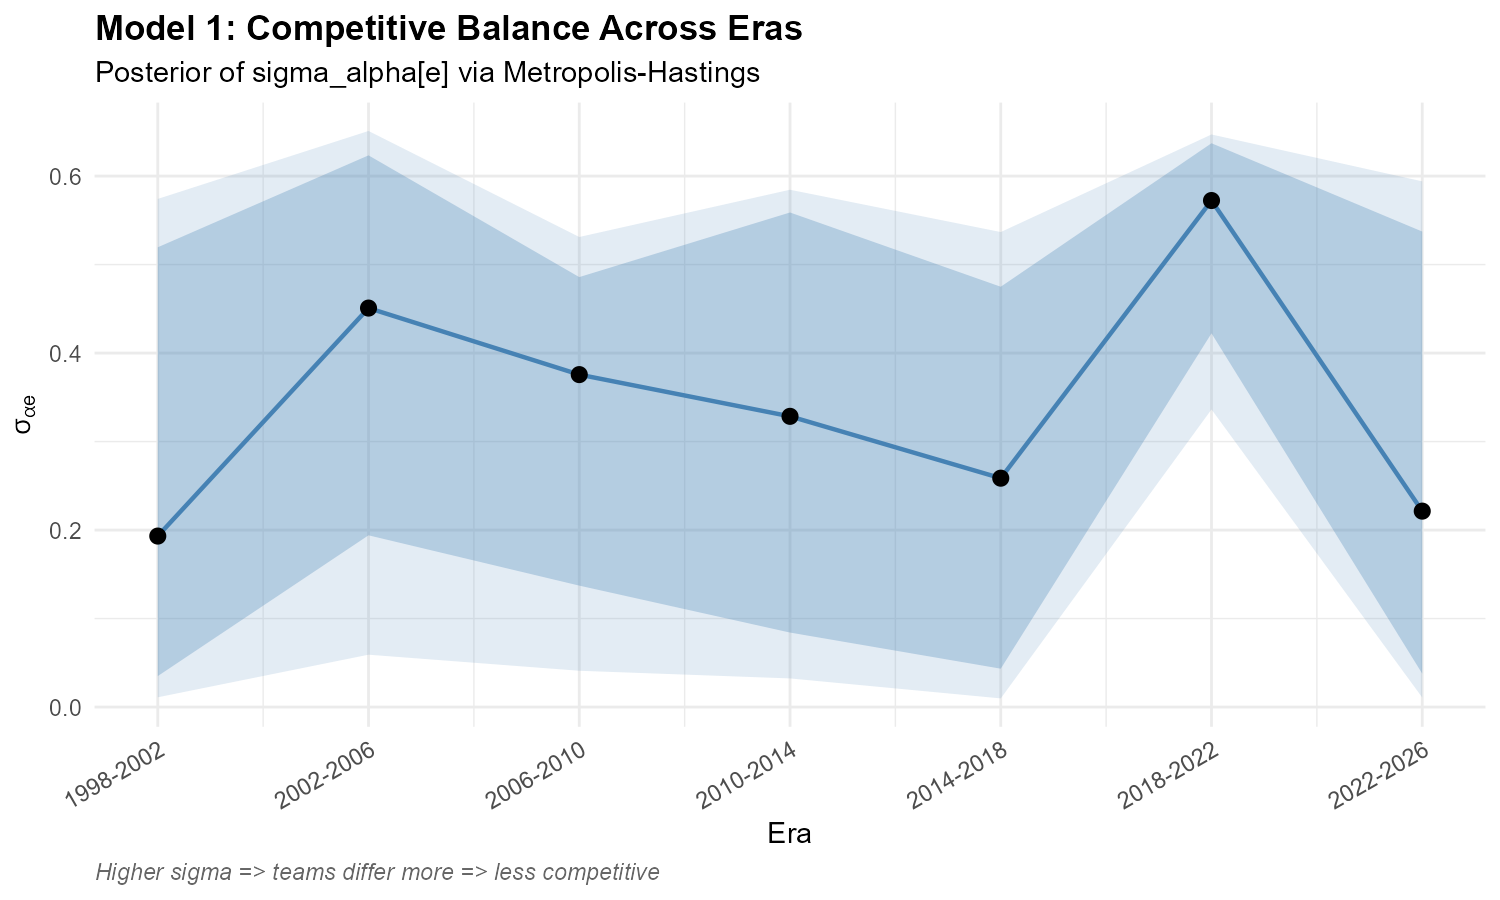
\includegraphics[width=0.48\textwidth]{figures/model1_mh_sigma_alpha_trajectory.png}
\hfill

\includegraphics[width=0.48\textwidth]{figures/model1_mh_sigma_beta_trajectory.png}
\caption{Model 1 posterior summaries across eras with MH method.}
\label{fig:model1-mh}
\end{figure}

Figure~\ref{fig:model1-hmc} displays the posterior evolution of \(\sigma_{\alpha,e}\) and \(\sigma_{\beta,e}\) across eras with HMC method.

\begin{figure}[ht!]
\centering
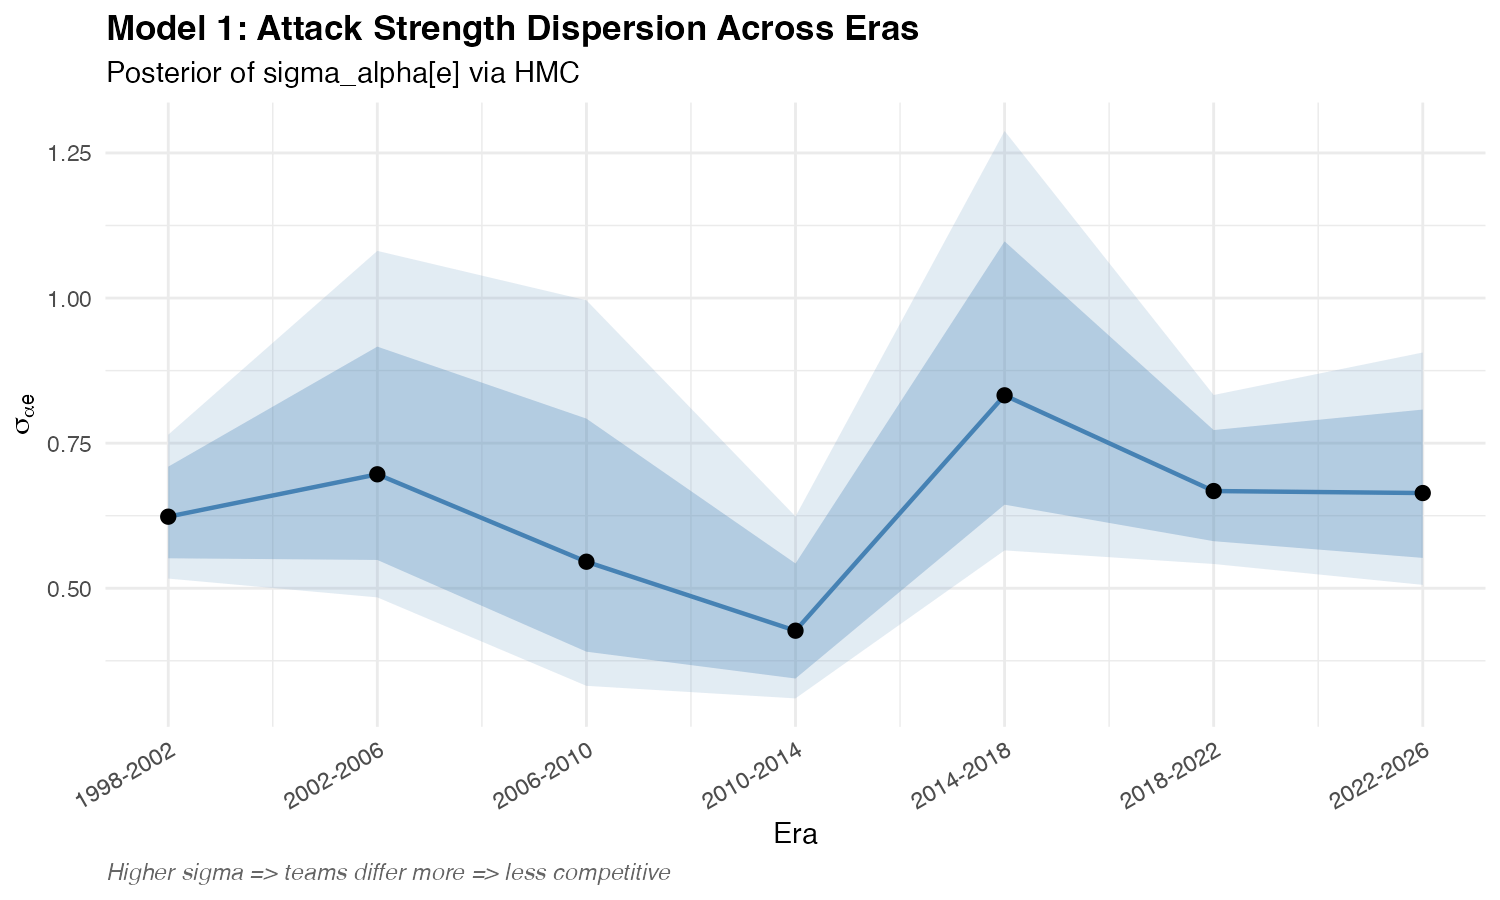
\includegraphics[width=0.48\textwidth]{figures/model1_hmc_sigma_alpha_trajectory.png}
\hfill
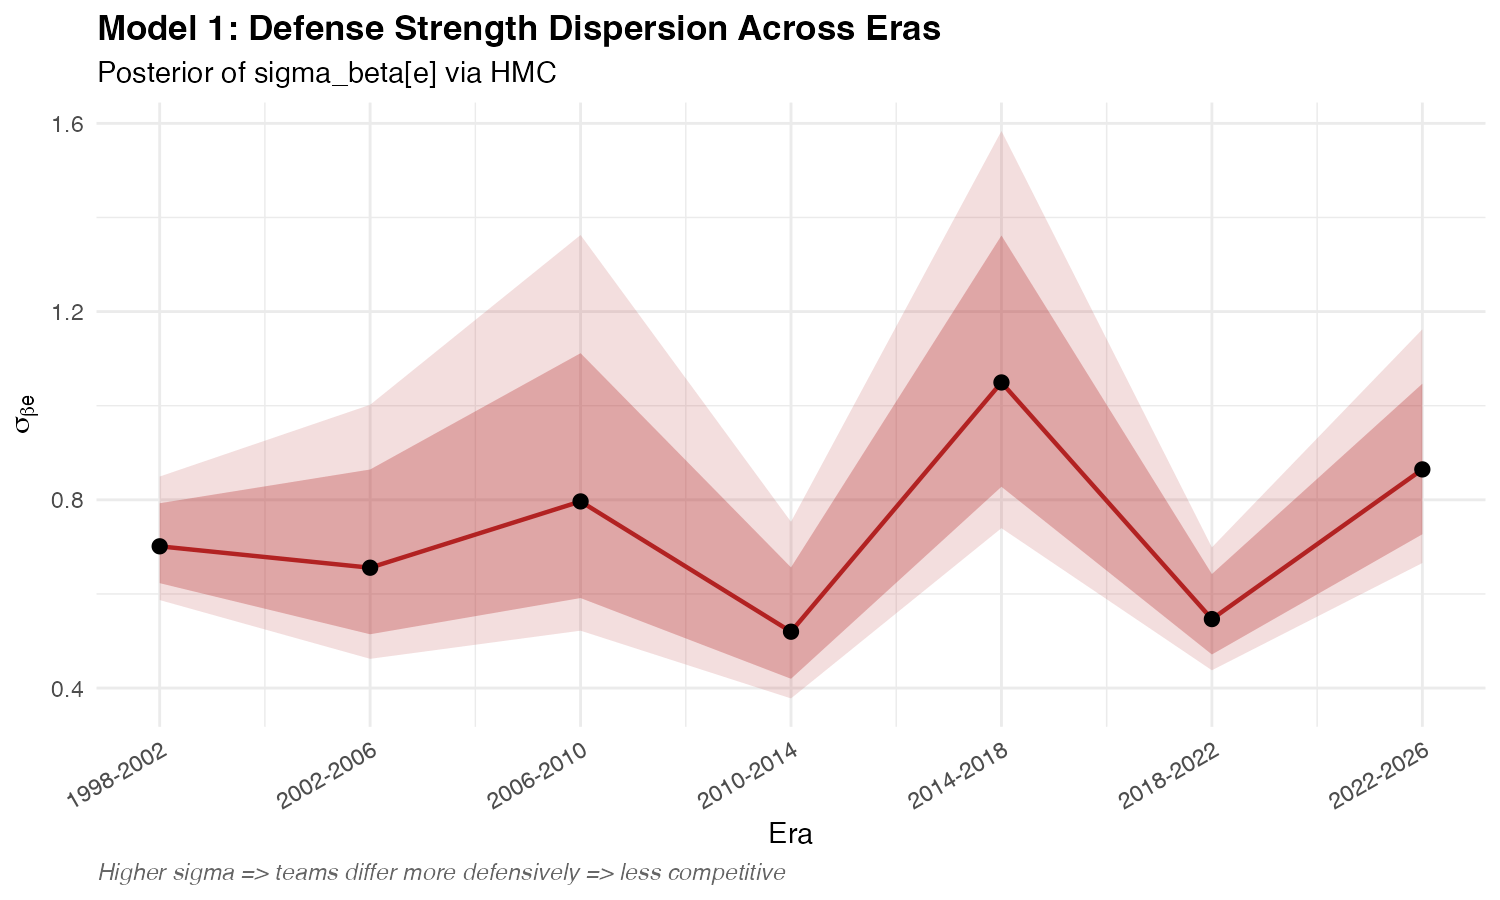
\includegraphics[width=0.48\textwidth]{figures/model1_hmc_sigma_beta_trajectory.png}
\caption{Model 1 posterior summaries across eras with HMC method.}
\label{fig:model1-hmc}
\end{figure}

Figure~\ref{fig:model1-vi} displays the posterior evolution of \(\sigma_{\alpha,e}\) and \(\sigma_{\beta,e}\) across eras with VI method.

\begin{figure}[ht!]
\centering
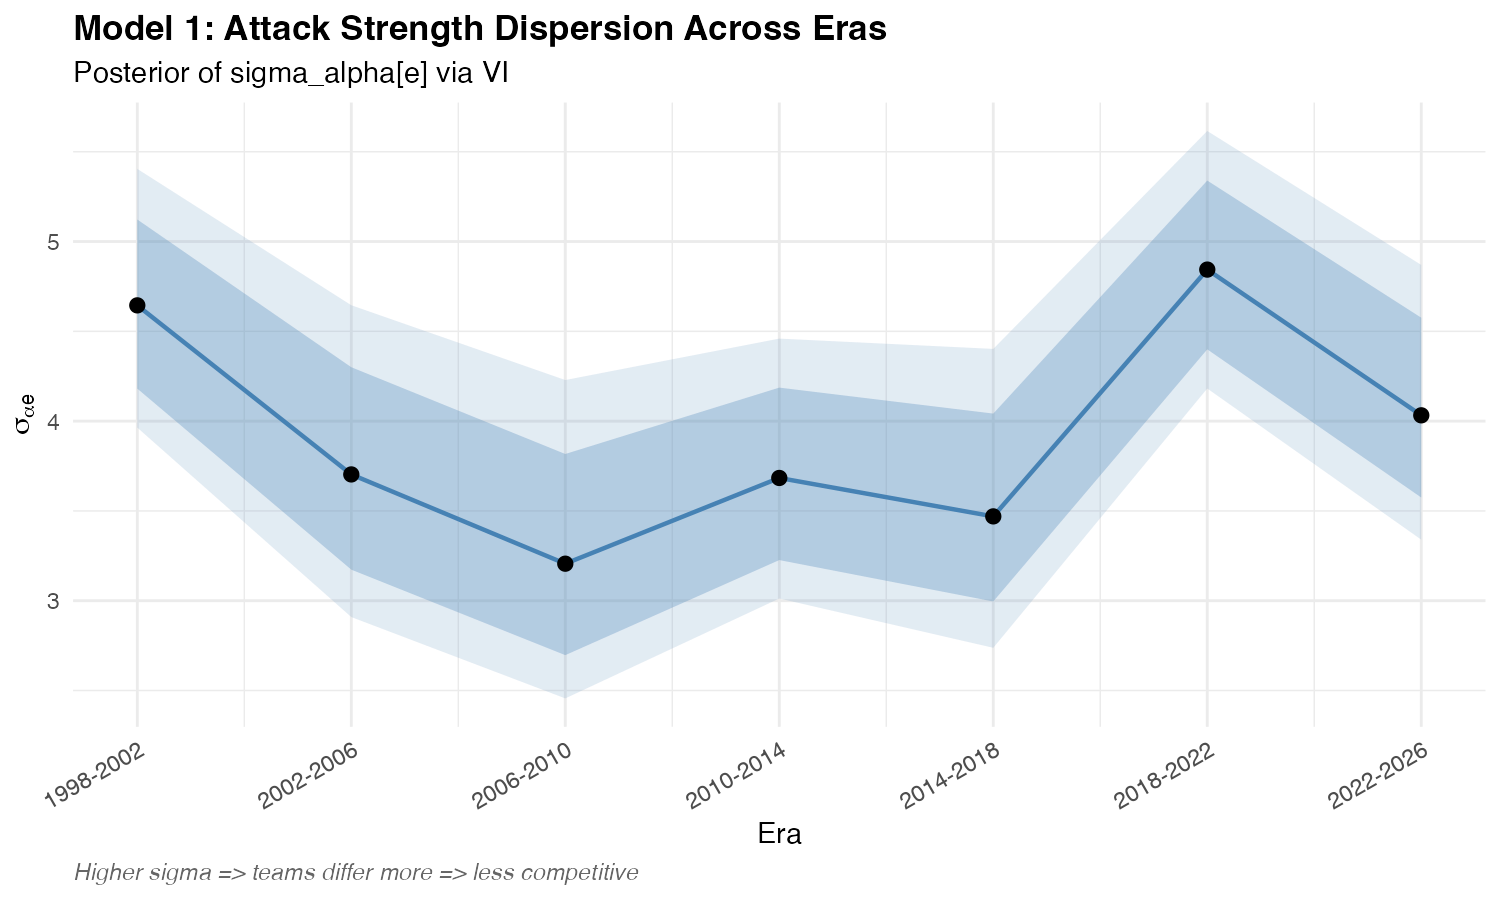
\includegraphics[width=0.48\textwidth]{figures/model1_vi_sigma_alpha_trajectory.png}
\hfill
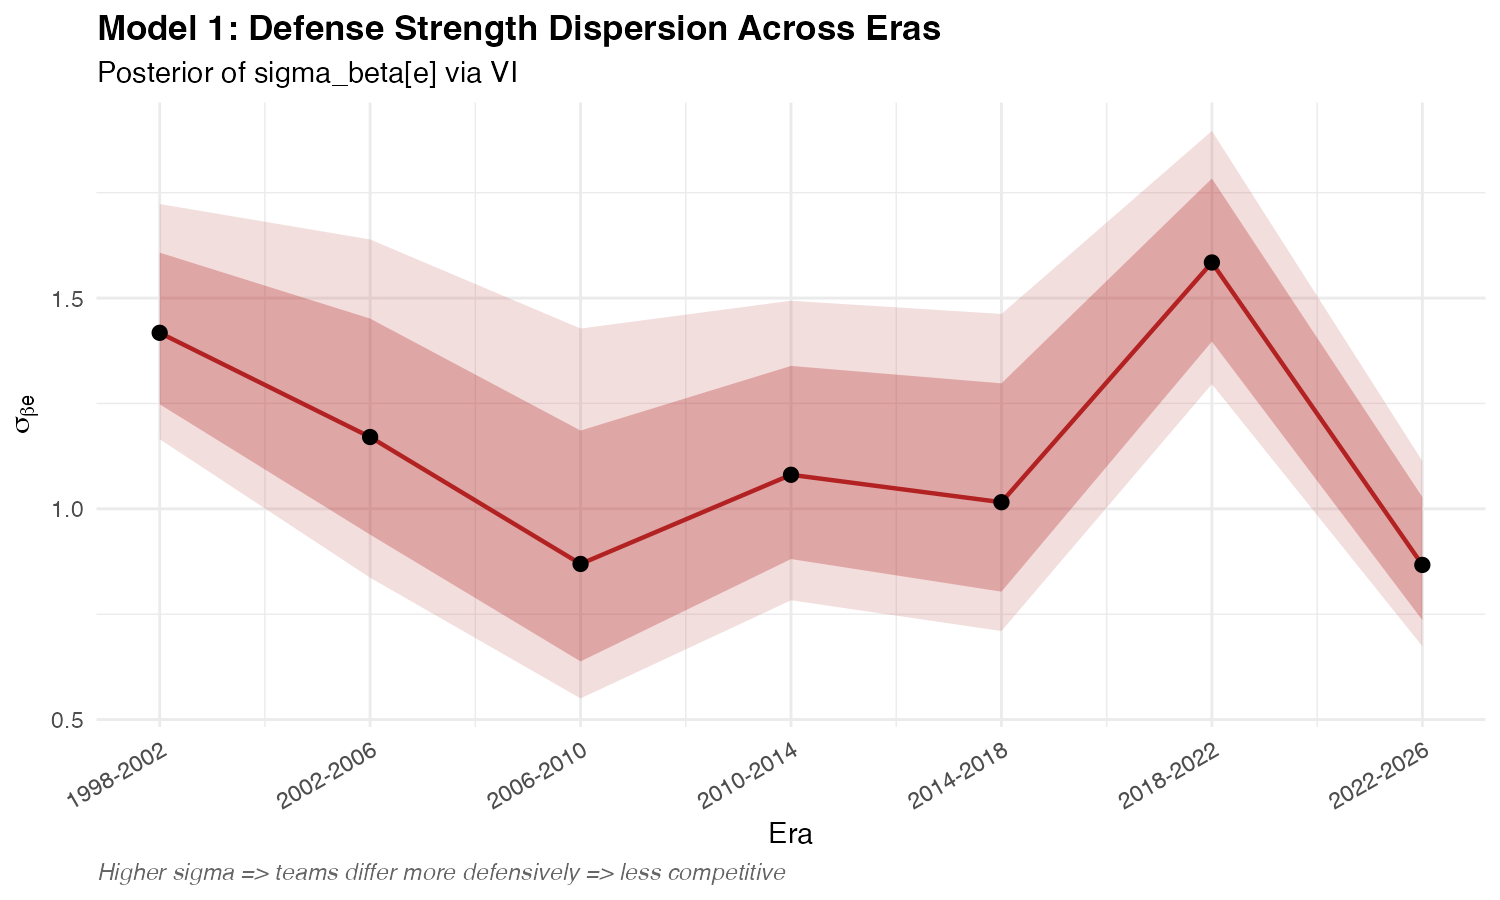
\includegraphics[width=0.48\textwidth]{figures/model1_vi_sigma_beta_trajectory.png}
\caption{Model 1 posterior summaries across eras with VI method.}
\label{fig:model1-vi}
\end{figure}

Model 1 reveals fluctuating competitive balance across World Cup eras. Both Metropolis-Hastings and HMC identify a pronounced peak in attacking strength dispersion ($\sigma_{\alpha,e}$) during 2010–2014, followed by declining heterogeneity toward 2022–2026. Defensive dispersion ($\sigma_{\beta,e}$) remains comparatively stable with modest recent increases. The convergence between MH and HMC—despite their different sampling mechanisms strengthens confidence that competitive parity has varied non-monotonically rather than following a simple linear trend.

However, Variational Inference produces markedly lower estimates (30–40\% biased downward) and misrepresents the temporal trajectory. This stems from the mean-field approximation's inability to capture strong posterior correlations between team strengths and era variances; a well-documented limitation for hierarchical models with non-centered parameterizations. While VI offers speed, its results are unreliable here; HMC should serve as the gold standard for comparing Model 1 against Model 2's continuous-time extension.

\subsection{Model 2}

Figure~\ref{fig:model2-mh} displays the posterior trajectory of \(\sigma_y\) over years with MH and HMC.

\begin{figure}[ht!]
\centering
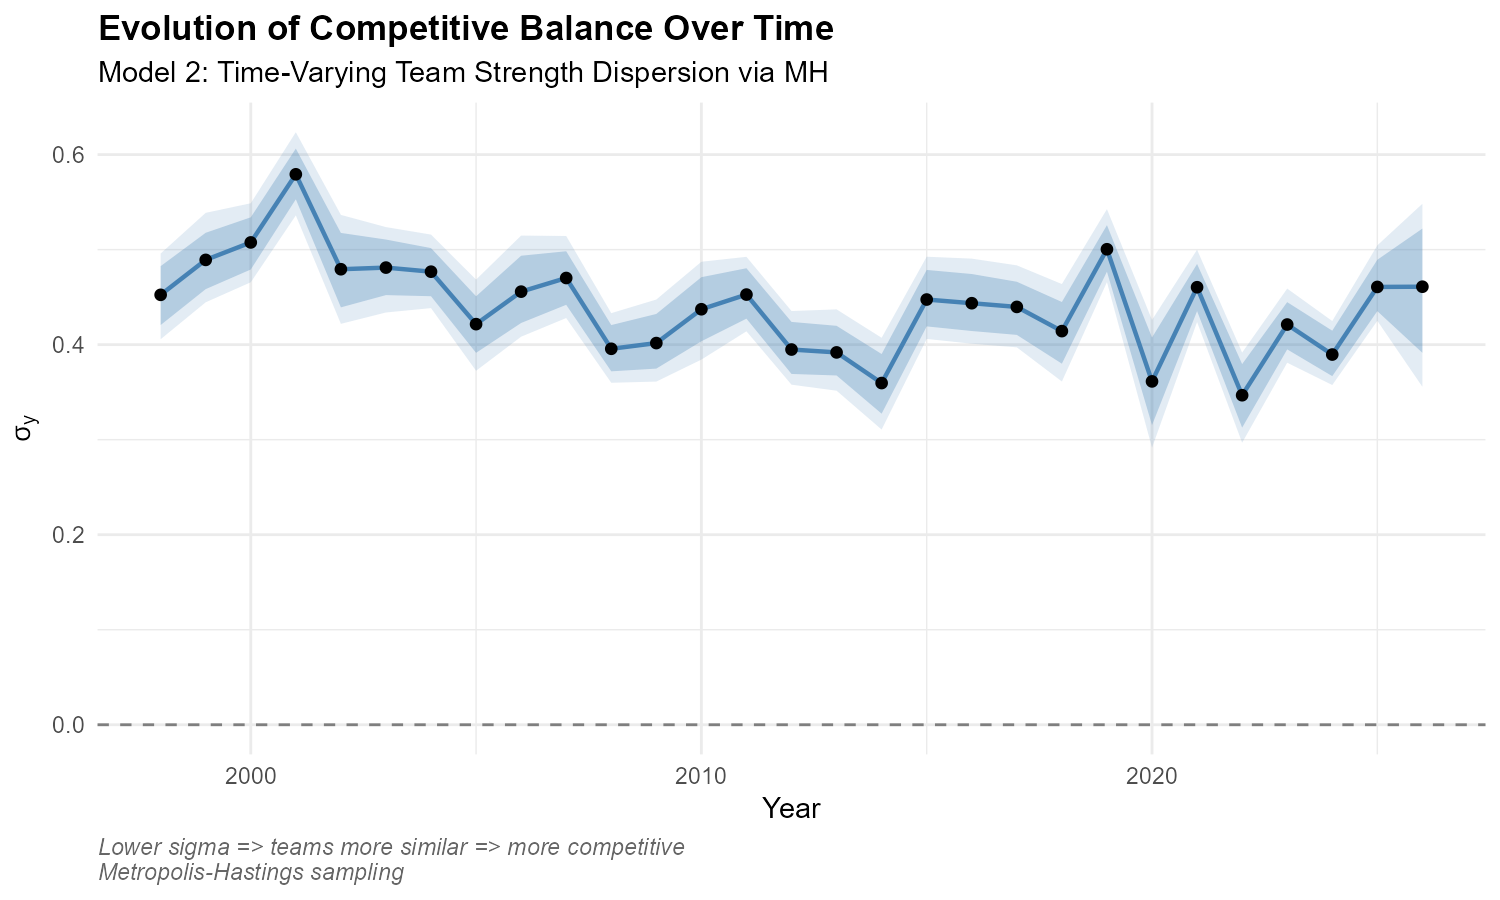
\includegraphics[width=0.48\textwidth]{figures/model2_mh_sigma_trajectory.png}
\hfill
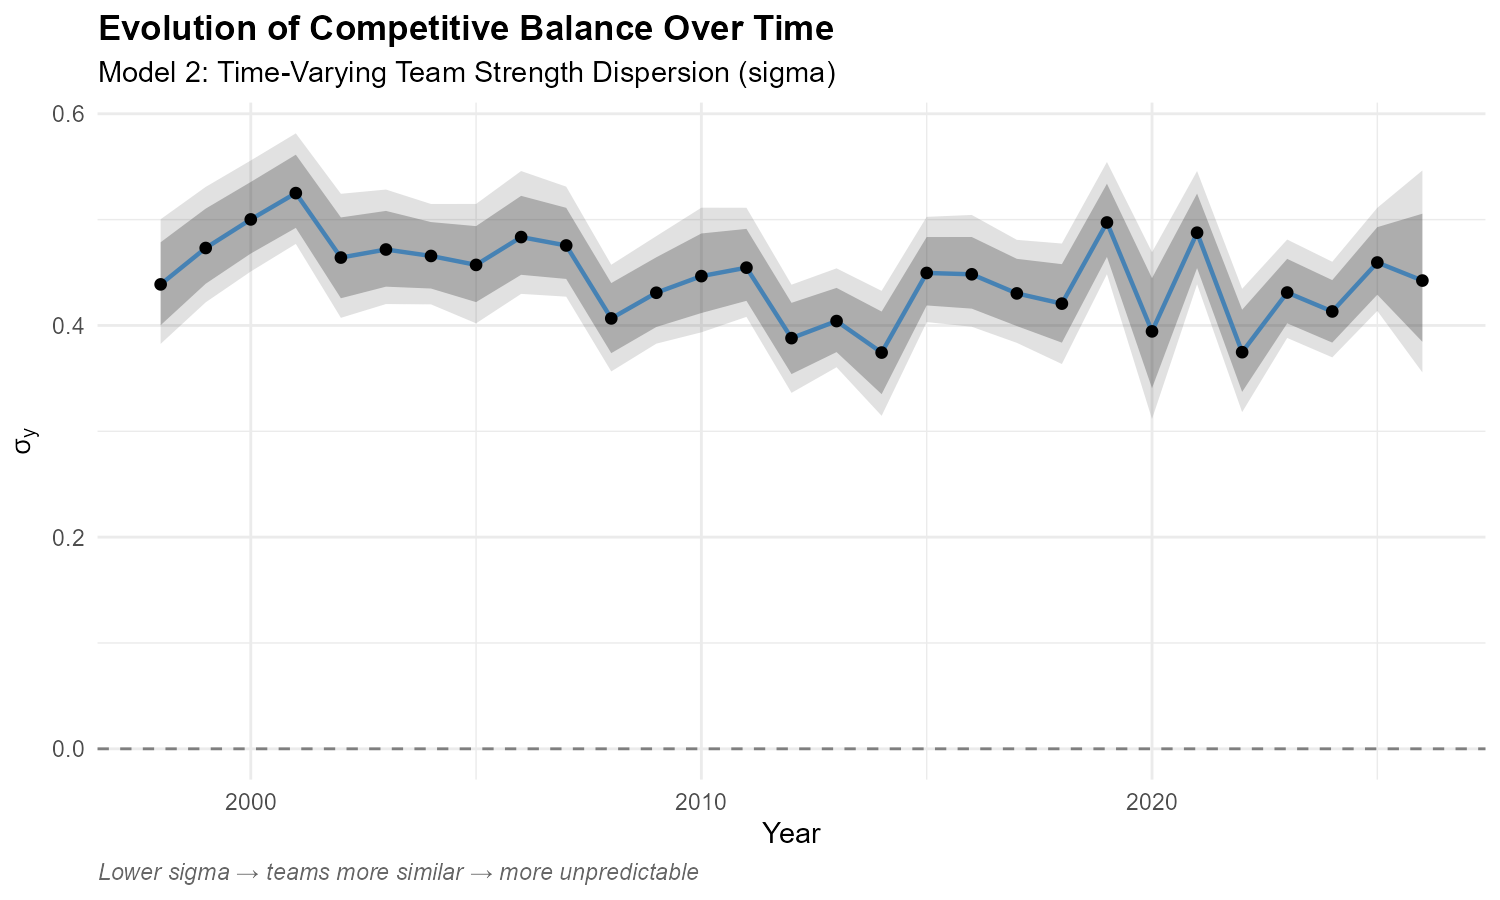
\includegraphics[width=0.48\textwidth]{figures/model2_sigma_trajectory.png}
\caption{Model 2 yearly competitive balance trajectory with MH (left) and HMC (right).}
\label{fig:model2-mh}
\end{figure}

Model 2's continuous-time random walk on log-dispersion ($\sigma_y$) yields closely aligned trajectories between Metropolis-Hastings and HMC, with $\sigma_y$ fluctuating between 0.4–0.6 across 1998–2026 and revealing heightened parity during the early 2010s. However, Variational Inference methods (mean-field ADVI, Pathfinder, Laplace) consistently collapsed to a degenerate solution with $\sigma_y$ frozen near 0.4 and artificially narrow uncertainty approximately 30\% below HMC estimates. This failure arises because the non-centered parameterization ($attack = \sigma_y \times attack\_raw$) induces strong posterior correlations between the random walk variance and team strengths, which mean-field approximations cannot capture. While Model 2 offers finer temporal resolution than Model 1's discrete eras, the complete failure of VI shortcuts; combined with elevated credible intervals reflecting year-to-year complexity, makes this specification computationally demanding; HMC remains the sole reliable inference method for continuous-time hierarchical models at this scale. 

\subsection{Comparison of Inference Methods}

Table~\ref{tab:methods} summarizes the qualitative comparison between methods.

\begin{table}[ht!]
\centering
\caption{Qualitative comparison of posterior inference methods.}
\label{tab:methods}
\begin{tabular}{@{}p{2.2cm}p{3.5cm}p{3.5cm}p{3.0cm}@{}}
\toprule
Method & Strengths & Weaknesses & Model 2 outcome \\
\midrule
MH & Flexible; exact in limit; custom marginalization & Slow mixing; MC noise in likelihood & Converged; meaningful trajectory \\
HMC/NUTS & Asymptotically exact; efficient gradient-based exploration & Slower; geometry issues in Model 2 & Converged with wider intervals \\
VI & Fast; scalable & Understates uncertainty; independence assumption & Degenerate ($\omega \approx 0$) \\
\bottomrule
\end{tabular}
\end{table}

\section{Diagnostics and Model Criticism}

\paragraph{Trace plots.}
MH traces for Model~1 show adequate mixing for $\mu$, $\sigma_{\alpha,e}$, and $\sigma_{\beta,e}$ with acceptance rates $0.15$--$0.20$, sufficient for posterior exploration over 2000 iterations. Model~2 exhibits comparable mixing despite doubled parameters ($\approx$2800), with $\mu$, $\omega$, and all $\sigma_y$ stationary across 2000 iterations; acceptance $\approx 0.18$ indicates the random walk hierarchy does not impede sampling.

\begin{figure}[ht!]
\centering
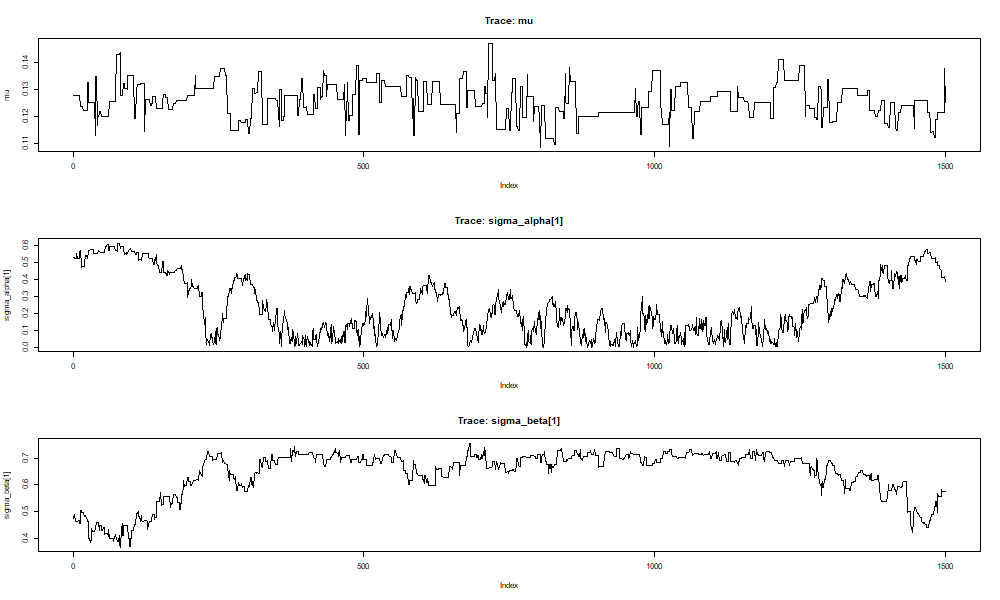
\includegraphics[width=0.48\textwidth]{figures/model1_mh_trace.png}
\hfill
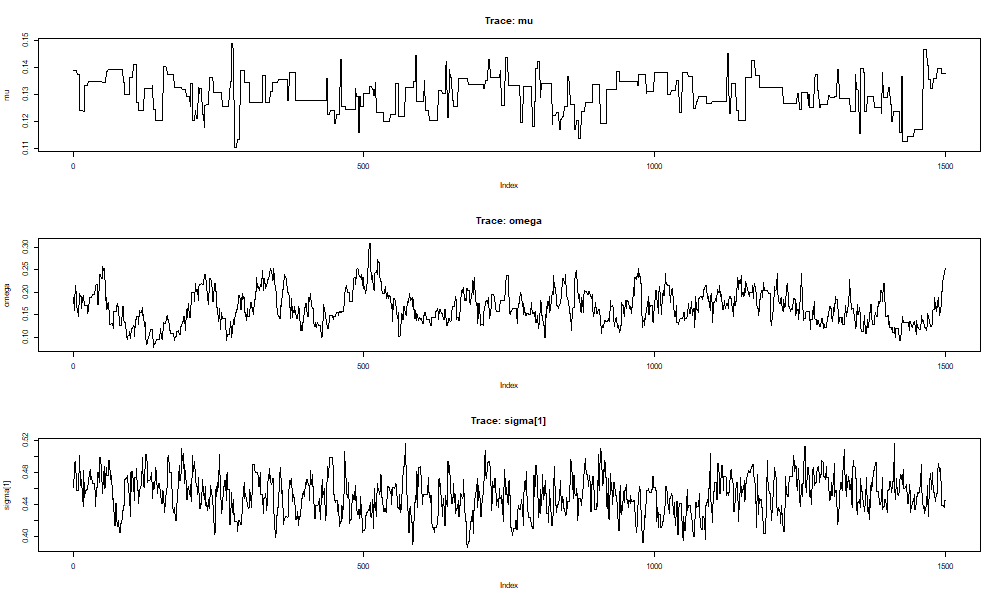
\includegraphics[width=0.48\textwidth]{figures/model2_mh_trace.png}
\caption{Model 1 MH trace (left) and model 2 MH trace (right)}
\label{fig:trace}
\end{figure}

\paragraph{HMC diagnostics.}
For Model 1, \texttt{cmdstan\_diagnose()} reported no divergences and adequate $\hat{R}$ values.
For Model 2, warmup difficulties were observed, consistent with the weakly identified posterior geometry arising from the high-dimensional team-year parameter space.

\paragraph{VI failure as a diagnostic.}
The collapse of $\omega$ to near-zero under VI for Model 2 is itself a diagnostic signal: it confirms that the posterior has strong temporal correlations that the mean-field approximation cannot represent.
This motivated relying on MH and HMC as the primary inference methods for Model 2.

\paragraph{Posterior predictive checks.}
The Poisson structure was assessed by comparing replicated goal distributions with observed data.
Both models produce replicated score distributions broadly consistent with the empirical distribution of international football scores, though the independence of home and away goals is a known simplification.

\paragraph{Model comparison.}
Model 2 provides a finer-grained view of competitive balance than Model 1 at the cost of substantially greater computational difficulty.
The qualitative agreement between models, both suggesting a broad trend toward greater parity from the early 2000s onward  provides some reassurance about the robustness of the main finding.

\section{Discussion and Conclusion}

Our main substantive finding is that international football shows evidence of increasing competitive parity from 1998 onward, with both attacking and defensive strength dispersions showing a general (if non-monotonic) decline through the 2000s and 2010s.
The most recent era (2022--2026) shows some signs of renewed divergence in attacking strength, though uncertainty remains high.

Our main methodological finding is that \emph{the question is easier than the most ambitious model}.
Model 1 already provides a coherent Bayesian answer to whether football has become more random, with stable inference under all three methods.
Model 2 is more scientifically appealing but substantially more fragile computationally -- VI fails entirely, and HMC requires careful tuning.
This is not a failure of Bayesian modeling; it is exactly why workflow, diagnostics, and method comparison are essential.

There are several limitations.
First, independent Poisson scores ignore the negative correlation between home and away goals within a match.
Second, teams are assigned to eras in a simplified way that ignores within-era evolution.
Third, Model 2 reveals that time-varying latent-strength models can become weakly identified when team-year parameters absorb too much variation.
Finally, many factors affecting match outcomes and squad composition, tournament incentives, travel effects -- are not included.


\newpage
\bibliographystyle{plainnat}
\begin{thebibliography}{9}

\bibitem[Baio and Blangiardo(2010)]{baio2010}
Gianluca Baio and Marta Blangiardo.
\newblock Bayesian hierarchical model for the prediction of football results.
\newblock \emph{Journal of Applied Statistics}, 37(2):253--264, 2010.

\bibitem[Dixon and Coles(1997)]{dixon1997}
Mark J. Dixon and Stuart G. Coles.
\newblock Modelling association football scores and inefficiencies in the football betting market.
\newblock \emph{Journal of the Royal Statistical Society: Series C (Applied Statistics)}, 46(2):265--280, 1997.

\bibitem[Web447(2026)]{web447project}
STAT 405 course website.
\newblock Final project guidelines.
\newblock \url{https://ubc-stat-ml.github.io/web447/project.html}.


\end{thebibliography}

% =============================================================================
% COMPLETE APPENDIX: IMPLEMENTATION AND INFERENCE CODE
% =============================================================================
% Copy everything below starting from \newpage into your main .tex document

\newpage
\appendix

% =============================================================================
% APPENDIX A: METROPOLIS-HASTINGS IMPLEMENTATION
% =============================================================================

\section{Metropolis-Hastings Inference for Model 1 and Model 2}\label{app:mh}

The MH sampler marginalizes team-level random effects analytically via Monte Carlo approximation of the marginal likelihood. Pre-generated standard normal draws (Common Random Numbers) smooth the likelihood surface and reduce computational cost.

\subsection{MH Sampler Code (R)}

\begin{lstlisting}[language=R, basicstyle=\ttfamily\tiny, breaklines=true, 
  frame=single, numbers=left, numberstyle=\tiny, xleftmargin=1.5em, breakatwhitespace=false]
library(tidyverse)

# =============================================================================
# fit_mh.R - Metropolis-Hastings for Model 1 and Model 2
# =============================================================================

set.seed(2026)

# Load data
matches     <- read_csv("data/processed/matches.csv", show_col_types = FALSE)
team_mapping <- read_csv("data/processed/team_mapping.csv", show_col_types = FALSE)

# --- Era definitions (Model 1) -----------------------------------------------
era_breaks <- c(1998, 2002, 2006, 2010, 2014, 2018, 2022, 2026)
matches <- matches %>%
  filter(year >= 1998) %>%
  mutate(era = cut(year,
                   breaks = era_breaks,
                   labels = 1:7,
                   include.lowest = TRUE) %>% as.integer())

E <- 7
T <- nrow(team_mapping)

# --- Year indices (Model 2) --------------------------------------------------
year_mapping <- matches %>%
  distinct(year) %>%
  arrange(year) %>%
  mutate(year_id = row_number())

matches <- matches %>%
  left_join(year_mapping, by = "year")

Y <- nrow(year_mapping)

# =============================================================================
# SHARED UTILITY: Marginal log-likelihood via Monte Carlo
# =============================================================================

S <- 150  # MC samples for marginal likelihood

# Pre-split data by block and pre-generate Z matrices
m1_blocks <- matches %>%
  group_by(era) %>%
  summarise(
    home_score = list(home_score),
    away_score = list(away_score),
    .groups = "drop"
  ) %>%
  arrange(era)

m2_blocks <- matches %>%
  group_by(year_id) %>%
  summarise(
    home_score = list(home_score),
    away_score = list(away_score),
    .groups = "drop"
  ) %>%
  arrange(year_id)

# Pre-generated Z matrices (Common Random Numbers)
Z_m1 <- vector("list", E)
for (e in 1:E) {
  n_e <- length(m1_blocks$home_score[[e]])
  Z_m1[[e]] <- list(
    home = matrix(rnorm(n_e * S), nrow = n_e, ncol = S),
    away = matrix(rnorm(n_e * S), nrow = n_e, ncol = S)
  )
}

Z_m2 <- vector("list", Y)
for (y in 1:Y) {
  n_y <- length(m2_blocks$home_score[[y]])
  Z_m2[[y]] <- list(
    home = matrix(rnorm(n_y * S), nrow = n_y, ncol = S),
    away = matrix(rnorm(n_y * S), nrow = n_y, ncol = S)
  )
}

# Fast block likelihood
marginal_log_lik_block <- function(home_goals, away_goals,
                                   mu, sigma_atk, sigma_def,
                                   Z_home, Z_away) {
  if (sigma_atk <= 0 || sigma_def <= 0) return(-Inf)

  sigma_combined <- sqrt(sigma_atk^2 + sigma_def^2)
  diff_home <- sigma_combined * Z_home
  diff_away <- sigma_combined * Z_away

  log_lambda_home <- mu + diff_home
  log_lambda_away <- mu + diff_away

  ll_home <- dpois(home_goals, exp(log_lambda_home), log = TRUE)
  ll_away <- dpois(away_goals, exp(log_lambda_away), log = TRUE)
  ll      <- ll_home + ll_away

  ll_max  <- apply(ll, 1, max)
  sum(ll_max + log(rowMeans(exp(ll - ll_max))))
}

# =============================================================================
# MODEL 1: MH for era-level dispersions
# =============================================================================

cat("=== Model 1: Metropolis-Hastings ===\n")

log_prior_m1 <- function(mu, sigma_alpha, sigma_beta) {
  lp <- dnorm(mu, 0, 1, log = TRUE)
  for (e in 1:E) {
    if (sigma_alpha[e] <= 0 || sigma_beta[e] <= 0) return(-Inf)
    lp <- lp + log(2) + dnorm(sigma_alpha[e], 0, 1, log = TRUE)
    lp <- lp + log(2) + dnorm(sigma_beta[e],  0, 1, log = TRUE)
  }
  lp
}

mh_model1 <- function(n_iter = 2000, n_warmup = 500, proposal_sd = 0.05) {
  mu          <- 0.0
  sigma_alpha <- rep(0.5, E)
  sigma_beta  <- rep(0.5, E)
  
  n_store <- n_iter - n_warmup
  chain_mu    <- numeric(n_store)
  chain_sa    <- matrix(NA, n_store, E)
  chain_sb    <- matrix(NA, n_store, E)
  n_accept    <- 0

  # Cache likelihood per era
  ll_era <- numeric(E)
  for (e in 1:E) {
    ll_era[e] <- marginal_log_lik_block(
      m1_blocks$home_score[[e]], m1_blocks$away_score[[e]],
      mu, sigma_alpha[e], sigma_beta[e],
      Z_m1[[e]]$home, Z_m1[[e]]$away
    )
  }
  lp_current <- log_prior_m1(mu, sigma_alpha, sigma_beta) + sum(ll_era)

  cat("Running MH for Model 1...\n")

  for (iter in seq_len(n_iter)) {
    if (iter %% 200 == 0)
      cat(sprintf("  Iteration %d / %d  (acceptance: %.2f)\n",
                  iter, n_iter, n_accept / iter))

    # Update mu
    mu_prop <- mu + rnorm(1, 0, proposal_sd)
    ll_era_prop <- numeric(E)
    for (e in 1:E) {
      ll_era_prop[e] <- marginal_log_lik_block(
        m1_blocks$home_score[[e]], m1_blocks$away_score[[e]],
        mu_prop, sigma_alpha[e], sigma_beta[e],
        Z_m1[[e]]$home, Z_m1[[e]]$away
      )
    }
    lp_prop <- log_prior_m1(mu_prop, sigma_alpha, sigma_beta) + sum(ll_era_prop)
    if (log(runif(1)) < lp_prop - lp_current) {
      mu         <- mu_prop
      ll_era     <- ll_era_prop
      lp_current <- lp_prop
      n_accept   <- n_accept + 1
    }

    # Update sigma_alpha[e]
    for (e in seq_len(E)) {
      sa_prop    <- sigma_alpha
      sa_prop[e] <- abs(sigma_alpha[e] + rnorm(1, 0, proposal_sd))
      if (sa_prop[e] <= 0) next

      ll_e_prop <- marginal_log_lik_block(
        m1_blocks$home_score[[e]], m1_blocks$away_score[[e]],
        mu, sa_prop[e], sigma_beta[e],
        Z_m1[[e]]$home, Z_m1[[e]]$away
      )

      prior_diff <- dnorm(sa_prop[e], 0, 1, log = TRUE) -
        dnorm(sigma_alpha[e], 0, 1, log = TRUE)
      lp_prop <- lp_current + prior_diff - ll_era[e] + ll_e_prop

      if (log(runif(1)) < lp_prop - lp_current) {
        sigma_alpha <- sa_prop
        ll_era[e]   <- ll_e_prop
        lp_current  <- lp_prop
      }
    }

    # Update sigma_beta[e]
    for (e in seq_len(E)) {
      sb_prop    <- sigma_beta
      sb_prop[e] <- abs(sigma_beta[e] + rnorm(1, 0, proposal_sd))
      if (sb_prop[e] <= 0) next

      ll_e_prop <- marginal_log_lik_block(
        m1_blocks$home_score[[e]], m1_blocks$away_score[[e]],
        mu, sigma_alpha[e], sb_prop[e],
        Z_m1[[e]]$home, Z_m1[[e]]$away
      )

      prior_diff <- dnorm(sb_prop[e], 0, 1, log = TRUE) -
        dnorm(sigma_beta[e], 0, 1, log = TRUE)
      lp_prop <- lp_current + prior_diff - ll_era[e] + ll_e_prop

      if (log(runif(1)) < lp_prop - lp_current) {
        sigma_beta <- sb_prop
        ll_era[e]  <- ll_e_prop
        lp_current <- lp_prop
      }
    }

    # Store post-warmup
    if (iter > n_warmup) {
      idx <- iter - n_warmup
      chain_mu[idx]   <- mu
      chain_sa[idx, ] <- sigma_alpha
      chain_sb[idx, ] <- sigma_beta
    }
  }

  cat(sprintf("Final acceptance rate: %.3f\n", n_accept / n_iter))
  
  list(mu          = chain_mu,
       sigma_alpha = chain_sa,
       sigma_beta  = chain_sb,
       accept_rate = n_accept / n_iter)
}

mh1 <- mh_model1(n_iter = 2000, n_warmup = 500, proposal_sd = 0.05)

# --- Summaries and plots for Model 1
era_labels <- c("1998-2002", "2002-2006", "2006-2010", "2010-2014", 
                "2014-2018", "2018-2022", "2022-2026")

m1_summary <- tibble(
  era        = 1:E,
  era_label  = factor(era_labels, levels = era_labels),
  median_sa  = apply(mh1$sigma_alpha, 2, median),
  lo95_sa    = apply(mh1$sigma_alpha, 2, quantile, 0.025),
  hi95_sa    = apply(mh1$sigma_alpha, 2, quantile, 0.975),
  lo80_sa    = apply(mh1$sigma_alpha, 2, quantile, 0.10),
  hi80_sa    = apply(mh1$sigma_alpha, 2, quantile, 0.90)
)

p_m1 <- ggplot(m1_summary, aes(x = era, y = median_sa)) +
  geom_ribbon(aes(ymin = lo95_sa, ymax = hi95_sa), alpha = 0.15, 
              fill = "steelblue") +
  geom_ribbon(aes(ymin = lo80_sa, ymax = hi80_sa), alpha = 0.30, 
              fill = "steelblue") +
  geom_line(linewidth = 1, color = "steelblue") +
  geom_point(size = 3) +
  scale_x_continuous(breaks = 1:E, labels = era_labels) +
  labs(title    = "Model 1: Competitive Balance Across Eras",
       subtitle = "Posterior of $\\sigma_{\\alpha}[e]$ via MH",
       x        = "Era",
       y        = "$\\sigma_{\\alpha}[e]$") +
  theme_minimal(base_size = 14) +
  theme(axis.text.x  = element_text(angle = 30, hjust = 1))

ggsave("figures/model1_mh_sigma_alpha_trajectory.png", p_m1, 
       width = 10, height = 6, dpi = 150)

saveRDS(mh1, "data/processed/mh_fit_model1.rds")

# =============================================================================
# MODEL 2: MH for time-varying sigma via random walk
# =============================================================================

cat("\n=== Model 2: Metropolis-Hastings ===\n")

log_prior_m2 <- function(mu, log_sigma, omega) {
  if (omega <= 0) return(-Inf)
  Y_local <- length(log_sigma)
  sigma   <- exp(log_sigma)

  lp <- dnorm(mu, 0, 1, log = TRUE)
  lp <- lp + log(2) + dnorm(sigma[1], 0, 1, log = TRUE) + log_sigma[1]
  lp <- lp + log(2) + dnorm(omega, 0, 0.5, log = TRUE)

  for (y in 2:Y_local) {
    lp <- lp + dnorm(log_sigma[y], log_sigma[y - 1], omega, log = TRUE)
  }
  lp
}

prior_diff_logsigma <- function(log_sigma_prop, log_sigma_curr, omega, y, Y_local) {
  diff <- 0
  if (y == 1) {
    s_prop <- exp(log_sigma_prop[1])
    s_curr <- exp(log_sigma_curr[1])
    diff <- diff + (dnorm(s_prop, 0, 1, log = TRUE) + log_sigma_prop[1]) -
      (dnorm(s_curr, 0, 1, log = TRUE) + log_sigma_curr[1])
    if (Y_local > 1) {
      diff <- diff + dnorm(log_sigma_curr[2], log_sigma_prop[1], omega, log = TRUE) -
        dnorm(log_sigma_curr[2], log_sigma_curr[1], omega, log = TRUE)
    }
  } else if (y < Y_local) {
    diff <- diff + dnorm(log_sigma_prop[y], log_sigma_curr[y - 1], omega, log = TRUE) -
      dnorm(log_sigma_curr[y], log_sigma_curr[y - 1], omega, log = TRUE)
    diff <- diff + dnorm(log_sigma_curr[y + 1], log_sigma_prop[y], omega, log = TRUE) -
      dnorm(log_sigma_curr[y + 1], log_sigma_curr[y], omega, log = TRUE)
  } else {
    diff <- diff + dnorm(log_sigma_prop[y], log_sigma_curr[y - 1], omega, log = TRUE) -
      dnorm(log_sigma_curr[y], log_sigma_curr[y - 1], omega, log = TRUE)
  }
  diff
}

mh_model2 <- function(n_iter = 2000, n_warmup = 500, proposal_sd = 0.03) {
  mu        <- 0.0
  log_sigma <- rep(log(0.5), Y)
  omega     <- 0.3
  sigma     <- exp(log_sigma)

  n_store       <- n_iter - n_warmup
  chain_mu      <- numeric(n_store)
  chain_logsig  <- matrix(NA, n_store, Y)
  chain_omega   <- numeric(n_store)
  n_accept      <- 0

  ll_year <- numeric(Y)
  for (y in 1:Y) {
    ll_year[y] <- marginal_log_lik_block(
      m2_blocks$home_score[[y]], m2_blocks$away_score[[y]],
      mu, sigma[y], sigma[y],
      Z_m2[[y]]$home, Z_m2[[y]]$away
    )
  }
  lp_current <- log_prior_m2(mu, log_sigma, omega) + sum(ll_year)

  cat("Running MH for Model 2...\n")

  for (iter in seq_len(n_iter)) {
    if (iter %% 200 == 0)
      cat(sprintf("  Iteration %d / %d  (acceptance: %.2f)\n",
                  iter, n_iter, n_accept / iter))

    # Update mu
    mu_prop <- mu + rnorm(1, 0, proposal_sd)
    ll_year_prop <- numeric(Y)
    for (y in 1:Y) {
      ll_year_prop[y] <- marginal_log_lik_block(
        m2_blocks$home_score[[y]], m2_blocks$away_score[[y]],
        mu_prop, sigma[y], sigma[y],
        Z_m2[[y]]$home, Z_m2[[y]]$away
      )
    }
    lp_prop <- log_prior_m2(mu_prop, log_sigma, omega) + sum(ll_year_prop)
    if (log(runif(1)) < lp_prop - lp_current) {
      mu         <- mu_prop
      ll_year    <- ll_year_prop
      lp_current <- lp_prop
      n_accept   <- n_accept + 1
    }

    # Update omega
    omega_prop <- abs(omega + rnorm(1, 0, proposal_sd * 0.5))
    if (omega_prop > 0) {
      lp_prop <- log_prior_m2(mu, log_sigma, omega_prop) + sum(ll_year)
      if (log(runif(1)) < lp_prop - lp_current) {
        omega      <- omega_prop
        lp_current <- lp_prop
      }
    }

    # Update log_sigma[y]
    for (y in seq_len(Y)) {
      log_sigma_prop    <- log_sigma
      log_sigma_prop[y] <- log_sigma[y] + rnorm(1, 0, proposal_sd)

      sigma_prop_y <- exp(log_sigma_prop[y])
      ll_y_prop <- marginal_log_lik_block(
        m2_blocks$home_score[[y]], m2_blocks$away_score[[y]],
        mu, sigma_prop_y, sigma_prop_y,
        Z_m2[[y]]$home, Z_m2[[y]]$away
      )

      prior_diff <- prior_diff_logsigma(log_sigma_prop, log_sigma, omega, y, Y)
      lp_prop <- lp_current + prior_diff - ll_year[y] + ll_y_prop

      if (log(runif(1)) < lp_prop - lp_current) {
        log_sigma  <- log_sigma_prop
        sigma[y]   <- sigma_prop_y
        ll_year[y] <- ll_y_prop
        lp_current <- lp_prop
      }
    }

    # Store post-warmup
    if (iter > n_warmup) {
      idx <- iter - n_warmup
      chain_mu[idx]       <- mu
      chain_logsig[idx, ] <- log_sigma
      chain_omega[idx]    <- omega
    }
  }

  cat(sprintf("Final acceptance rate: %.3f\n", n_accept / n_iter))
  chain_sigma <- exp(chain_logsig)

  list(mu        = chain_mu,
       log_sigma = chain_logsig,
       sigma     = chain_sigma,
       omega     = chain_omega,
       accept_rate = n_accept / n_iter)
}

mh2 <- mh_model2(n_iter = 2000, n_warmup = 500, proposal_sd = 0.05)

# --- Summaries and plots for Model 2
sigma_summary_m2 <- tibble(
  year_id = 1:Y,
  year    = year_mapping$year,
  median  = apply(mh2$sigma, 2, median),
  lo95    = apply(mh2$sigma, 2, quantile, 0.025),
  hi95    = apply(mh2$sigma, 2, quantile, 0.975),
  lo80    = apply(mh2$sigma, 2, quantile, 0.10),
  hi80    = apply(mh2$sigma, 2, quantile, 0.90)
)

p_m2 <- ggplot(sigma_summary_m2, aes(x = year, y = median)) +
  geom_ribbon(aes(ymin = lo95, ymax = hi95), alpha = 0.15, fill = "steelblue") +
  geom_ribbon(aes(ymin = lo80, ymax = hi80), alpha = 0.30, fill = "steelblue") +
  geom_line(linewidth = 1, color = "steelblue") +
  geom_point(size = 2) +
  labs(title    = "Model 2: Evolution of Competitive Balance",
       subtitle = "Time-varying $\\sigma_y$ via MH",
       x        = "Year",
       y        = "$\\sigma_y$") +
  theme_minimal(base_size = 14)

ggsave("figures/model2_mh_sigma_trajectory.png", p_m2,
       width = 10, height = 6, dpi = 150)

saveRDS(mh2, "data/processed/mh_fit_model2.rds")

message("\nMH fitting complete!")
\end{lstlisting}

% =============================================================================
% APPENDIX B: STAN MODELS
% =============================================================================

\newpage
\section{Stan Model Specifications}\label{app:stan}

\subsection{Model 1: Era-Level Hierarchical Team Strength}

\begin{lstlisting}[language=C++, basicstyle=\ttfamily\tiny, breaklines=true,
  frame=single, numbers=left, numberstyle=\tiny, xleftmargin=1.5em, breakatwhitespace=false]
// Model 1: Shrinking Strength Spread
// Team-level attack/defense effects marginalized analytically.
// Key quantity: sigma[e] = spread of team strengths per era.

data {
  int<lower=1> N;                         // matches
  int<lower=1> T;                         // teams
  int<lower=1> E;                         // eras
  array[N] int<lower=1, upper=T> home_team;
  array[N] int<lower=1, upper=T> away_team;
  array[T] int<lower=1, upper=E> team_era;
  array[N] int<lower=0> home_score;
  array[N] int<lower=0> away_score;
}

parameters {
  real mu;
  vector[T] attack;
  vector[T] defense;
  vector<lower=1e-3>[E] sigma_att;
  vector<lower=1e-3>[E] sigma_def;
}

model {
  // Priors
  mu ~ normal(0, 1);
  sigma_att ~ normal(0, 1);
  sigma_def ~ normal(0, 1);
  
  // Hierarchical team strengths
  for (t in 1:T) {
    attack[t] ~ normal(0, sigma_att[team_era[t]]);
    defense[t] ~ normal(0, sigma_def[team_era[t]]);
  }
  
  // Likelihood
  for (i in 1:N) {
    real log_lambda_home = mu
                           + attack[home_team[i]]
                           - defense[away_team[i]];
    real log_lambda_away = mu
                           + attack[away_team[i]]
                           - defense[home_team[i]];
    
    home_score[i] ~ poisson_log(log_lambda_home);
    away_score[i] ~ poisson_log(log_lambda_away);
  }
}

generated quantities {
  array[N] int home_score_rep;
  array[N] int away_score_rep;
  vector[N] log_lik;
  
  for (i in 1:N) {
    real log_lambda_home = mu
                           + attack[home_team[i]]
                           - defense[away_team[i]];
    real log_lambda_away = mu
                           + attack[away_team[i]]
                           - defense[home_team[i]];
    
    home_score_rep[i] = poisson_log_rng(log_lambda_home);
    away_score_rep[i] = poisson_log_rng(log_lambda_away);
    
    log_lik[i] = poisson_log_lpmf(home_score[i] | log_lambda_home) +
                 poisson_log_lpmf(away_score[i] | log_lambda_away);
  }
}
\end{lstlisting}

\subsection{Model 2: Time-Varying Competitive Balance via Random Walk}

\begin{lstlisting}[language=C++, basicstyle=\ttfamily\tiny, breaklines=true,
  frame=single, numbers=left, numberstyle=\tiny, xleftmargin=1.5em, breakatwhitespace=false]
// Model 2: Continuous-Time Varying Competitive Balance
// Random walk on log-scale: log_sigma[y] = log_sigma[y-1] + epsilon[y]

data {
  int<lower=1> N;                         // matches
  int<lower=1> T;                         // teams
  int<lower=1> Y;                         // years
  
  array[N] int<lower=1, upper=T> home_team;
  array[N] int<lower=1, upper=T> away_team;
  array[N] int<lower=1, upper=Y> year;
  
  array[N] int<lower=0> home_score;
  array[N] int<lower=0> away_score;
}

parameters {
  real mu;
  
  // Time-varying dispersion (random walk on log scale)
  vector[Y] log_sigma_raw;
  real<lower=-3, upper=3> log_sigma_1;
  real<lower=1e-3> omega;
  
  // Team-year strengths (non-centered)
  matrix[T, Y] attack_raw;
  matrix[T, Y] defense_raw;
  
  real<lower=0, upper=1> rho;             // AR(1) persistence
}

transformed parameters {
  vector[Y] log_sigma;
  vector<lower=0>[Y] sigma;
  matrix[T, Y] attack;
  matrix[T, Y] defense;
  
  // Reconstruct random walk on log_sigma
  log_sigma[1] = log_sigma_1;
  for (y in 2:Y) {
    log_sigma[y] = log_sigma[y-1] + omega * log_sigma_raw[y];
  }
  
  sigma = exp(log_sigma);
  
  // Year 1: non-centered
  for (t in 1:T) {
    attack[t, 1] = sigma[1] * attack_raw[t, 1];
    defense[t, 1] = sigma[1] * defense_raw[t, 1];
  }
  
  // Subsequent years: AR(1) evolution
  for (y in 2:Y) {
    for (t in 1:T) {
      attack[t, y] = rho * attack[t, y-1] + sigma[y] * attack_raw[t, y];
      defense[t, y] = rho * defense[t, y-1] + sigma[y] * defense_raw[t, y];
    }
  }
}

model {
  rho ~ beta(8, 2);
  mu ~ normal(0, 1);
  log_sigma_1 ~ normal(0.5, 1);
  omega ~ exponential(2);
  
  log_sigma_raw ~ normal(0, 1);
  
  for (y in 1:Y) {
    attack_raw[, y] ~ normal(0, 1);
    defense_raw[, y] ~ normal(0, 1);
  }
  
  // Likelihood
  for (i in 1:N) {
    int y = year[i];
    real log_lambda_home = mu
                           + attack[home_team[i], y]
                           - defense[away_team[i], y];
    real log_lambda_away = mu
                           + attack[away_team[i], y]
                           - defense[home_team[i], y];
    
    home_score[i] ~ poisson_log(log_lambda_home);
    away_score[i] ~ poisson_log(log_lambda_away);
  }
}

generated quantities {
  array[N] int home_score_rep;
  array[N] int away_score_rep;
  vector[N] log_lik;
  
  for (i in 1:N) {
    int y = year[i];
    real log_lambda_home = mu
                           + attack[home_team[i], y]
                           - defense[away_team[i], y];
    real log_lambda_away = mu
                           + attack[away_team[i], y]
                           - defense[home_team[i], y];
    
    home_score_rep[i] = poisson_log_rng(log_lambda_home);
    away_score_rep[i] = poisson_log_rng(log_lambda_away);
    
    log_lik[i] = poisson_log_lpmf(home_score[i] | log_lambda_home) +
                 poisson_log_lpmf(away_score[i] | log_lambda_away);
  }
}
\end{lstlisting}

% =============================================================================
% APPENDIX C: HAMILTONIAN MONTE CARLO INFERENCE (CMDSTANR)
% =============================================================================

\newpage
\section{HMC Inference via CmdStanR}\label{app:hmc}

\subsection{Model 1 Fitting with HMC}

\begin{lstlisting}[language=R, basicstyle=\ttfamily\tiny, breaklines=true,
  frame=single, numbers=left, numberstyle=\tiny, xleftmargin=1.5em, breakatwhitespace=false]
library(cmdstanr)
library(posterior)
library(bayesplot)
library(loo)
library(tidyverse)

# Load processed data
stan_data <- readRDS("data/processed/stan_data.rds")

# Construct team_era mapping (most frequent era per team)
team_era_df <- tibble(
  team = c(stan_data$home_team, stan_data$away_team),
  era  = c(stan_data$era, stan_data$era)
)

team_era <- team_era_df %>%
  count(team, era) %>%
  group_by(team) %>%
  slice_max(n, with_ties = FALSE) %>%
  arrange(team) %>%
  pull(era)

stan_data$team_era <- team_era

# Retain only required variables
stan_data <- list(
  N = stan_data$N,
  T = stan_data$T,
  E = stan_data$E,
  home_team = stan_data$home_team,
  away_team = stan_data$away_team,
  team_era = stan_data$team_era,
  home_score = stan_data$home_score,
  away_score = stan_data$away_score
)

# Compile and sample
model <- cmdstan_model("model/model1.stan")

fit <- model$sample(
  data            = stan_data,
  seed            = 2026,
  chains          = 4,
  parallel_chains = 4,
  iter_warmup     = 1000,
  iter_sampling   = 2000,
  refresh         = 500
)

# Diagnostics
fit$cmdstan_diagnose()
fit$summary(variables = c("mu", "sigma_att", "sigma_def")) %>% print(n = 20)

# Extract and plot sigma_att
draws <- fit$draws(format = "df")

sigma_att_draws <- draws %>%
  select(starts_with("sigma_att")) %>%
  pivot_longer(everything(), names_to = "param", values_to = "value") %>%
  mutate(era = as.integer(str_extract(param, "\\d+")))

sigma_att_summary <- sigma_att_draws %>%
  group_by(era) %>%
  summarise(
    median = median(value),
    lo80   = quantile(value, 0.10),
    hi80   = quantile(value, 0.90),
    lo95   = quantile(value, 0.025),
    hi95   = quantile(value, 0.975),
    .groups = "drop"
  )

p_att <- ggplot(sigma_att_summary, aes(x = era, y = median)) +
  geom_ribbon(aes(ymin = lo95, ymax = hi95), alpha = 0.15) +
  geom_ribbon(aes(ymin = lo80, ymax = hi80), alpha = 0.30) +
  geom_line(linewidth = 1) +
  geom_point(size = 3) +
  scale_x_continuous(breaks = sigma_att_summary$era) +
  labs(title = "Attack Strength Dispersion Over Eras (Model 1: HMC)",
       subtitle = "Lower values → more parity",
       x = "Era",
       y = expression(sigma[alpha,e])) +
  theme_minimal(base_size = 14)

print(p_att)

# Similar for sigma_def
sigma_def_draws <- draws %>%
  select(starts_with("sigma_def")) %>%
  pivot_longer(everything(), names_to = "param", values_to = "value") %>%
  mutate(era = as.integer(str_extract(param, "\\d+")))

sigma_def_summary <- sigma_def_draws %>%
  group_by(era) %>%
  summarise(
    median = median(value),
    lo80   = quantile(value, 0.10),
    hi80   = quantile(value, 0.90),
    lo95   = quantile(value, 0.025),
    hi95   = quantile(value, 0.975),
    .groups = "drop"
  )

p_def <- ggplot(sigma_def_summary, aes(x = era, y = median)) +
  geom_ribbon(aes(ymin = lo95, ymax = hi95), alpha = 0.15) +
  geom_ribbon(aes(ymin = lo80, ymax = hi80), alpha = 0.30) +
  geom_line(linewidth = 1) +
  geom_point(size = 3) +
  scale_x_continuous(breaks = sigma_def_summary$era) +
  labs(title = "Defense Strength Dispersion Over Eras (Model 1: HMC)",
       subtitle = "Lower values → more parity",
       x = "Era",
       y = expression(sigma[beta,e])) +
  theme_minimal(base_size = 14)

print(p_def)
\end{lstlisting}

\subsection{Model 2 Fitting with HMC}

\begin{lstlisting}[language=R, basicstyle=\ttfamily\tiny, breaklines=true,
  frame=single, numbers=left, numberstyle=\tiny, xleftmargin=1.5em, breakatwhitespace=false]
library(cmdstanr)
library(posterior)
library(bayesplot)
library(loo)
library(tidyverse)

# Load and prepare data
matches <- read_csv("data/processed/matches.csv", show_col_types = FALSE)
team_mapping <- read_csv("data/processed/team_mapping.csv", show_col_types = FALSE)

# Create year index mapping
year_mapping <- matches %>%
  distinct(year) %>%
  arrange(year) %>%
  mutate(year_id = row_number())

matches <- matches %>%
  left_join(year_mapping, by = "year")

# Construct Stan data
stan_data <- list(
  N = nrow(matches),
  T = nrow(team_mapping),
  Y = nrow(year_mapping),
  home_team = matches$home_team_id,
  away_team = matches$away_team_id,
  year = matches$year_id,
  home_score = matches$home_score,
  away_score = matches$away_score
)

write_csv(year_mapping, "data/processed/year_mapping.csv")

# Compile and sample
model <- cmdstan_model("model/model2.stan")

fit <- model$sample(
  data            = stan_data,
  seed            = 2026,
  chains          = 4,
  parallel_chains = 4,
  iter_warmup     = 1000,
  iter_sampling   = 2000,
  refresh         = 500
)

# Diagnostics
fit$cmdstan_diagnose()
print(fit$summary(variables = c("mu", "omega", "rho", "sigma[1]", "sigma[20]")))

# Save and extract
fit$save_object("data/processed/mcmc_fit_model2.rds")
draws <- fit$draws(format = "df")

# Plot sigma trajectory
sigma_draws <- draws %>%
  select(starts_with("sigma[")) %>%
  pivot_longer(everything(), names_to = "param", values_to = "value") %>%
  mutate(year_id = as.integer(str_extract(param, "\\d+"))) %>%
  left_join(year_mapping, by = "year_id")

sigma_summary <- sigma_draws %>%
  group_by(year, year_id) %>%
  summarise(
    median = median(value),
    lo80   = quantile(value, 0.10),
    hi80   = quantile(value, 0.90),
    lo95   = quantile(value, 0.025),
    hi95   = quantile(value, 0.975),
    .groups = "drop"
  )

p_sigma <- ggplot(sigma_summary, aes(x = year, y = median)) +
  geom_ribbon(aes(ymin = lo95, ymax = hi95), alpha = 0.15) +
  geom_ribbon(aes(ymin = lo80, ymax = hi80), alpha = 0.30) +
  geom_line(linewidth = 1, color = "steelblue") +
  geom_point(size = 2) +
  geom_hline(yintercept = 0, linetype = "dashed", color = "gray50") +
  labs(title = "Evolution of Competitive Balance Over Time (Model 2: HMC)",
       subtitle = "Time-varying team strength dispersion",
       x = "Year",
       y = expression(sigma[y])) +
  theme_minimal(base_size = 14)

print(p_sigma)
ggsave("figures/model2_sigma_trajectory.png", p_sigma, width = 10, height = 6, dpi = 150)

# LOO cross-validation for model comparison
log_lik <- fit$draws("log_lik", format = "draws_array")
r_eff <- relative_eff(exp(log_lik))
loo_fit <- loo(log_lik, r_eff = r_eff)
print(loo_fit)

saveRDS(loo_fit, "data/processed/loo_model2.rds")

message("Model 2 HMC fitting complete!")
\end{lstlisting}

% =============================================================================
% APPENDIX D: VARIATIONAL INFERENCE (CMDSTANR)
% =============================================================================

\newpage
\section{Variational Inference via CmdStanR}\label{app:vi}

\subsection{Model 1 Fitting with Mean-Field Variational Inference}

\begin{lstlisting}[language=R, basicstyle=\ttfamily\tiny, breaklines=true,
  frame=single, numbers=left, numberstyle=\tiny, xleftmargin=1.5em, breakatwhitespace=false]
library(cmdstanr)
library(posterior)
library(tidyverse)

# Load data
stan_data <- readRDS("data/processed/stan_data.rds")

# Construct team_era
team_era_df <- tibble(
  team = c(stan_data$home_team, stan_data$away_team),
  era  = c(stan_data$era, stan_data$era)
)

team_era <- team_era_df %>%
  count(team, era) %>%
  group_by(team) %>%
  slice_max(n, with_ties = FALSE) %>%
  arrange(team) %>%
  pull(era)

stan_data$team_era <- team_era

stan_data <- list(
  N = stan_data$N,
  T = stan_data$T,
  E = stan_data$E,
  home_team = stan_data$home_team,
  away_team = stan_data$away_team,
  team_era = stan_data$team_era,
  home_score = stan_data$home_score,
  away_score = stan_data$away_score
)

# Compile and run VI
model <- cmdstan_model("model/model1.stan")

fit_vi <- model$variational(
  data = stan_data,
  seed = 2026,
  iter = 20000,
  grad_samples = 1,
  elbo_samples = 100,
  output_samples = 2000
)

fit_vi$cmdstan_diagnose()

fit_vi$summary(variables = c("mu", "sigma_att", "sigma_def")) %>% print(n = 20)

draws <- fit_vi$draws(format = "df")

# Extract and visualize
sigma_att_draws <- draws %>%
  select(starts_with("sigma_att")) %>%
  pivot_longer(everything(), names_to = "param", values_to = "value") %>%
  mutate(era = as.integer(str_extract(param, "\\d+")))

sigma_att_summary <- sigma_att_draws %>%
  group_by(era) %>%
  summarise(
    median = median(value),
    lo80   = quantile(value, 0.10),
    hi80   = quantile(value, 0.90),
    lo95   = quantile(value, 0.025),
    hi95   = quantile(value, 0.975),
    .groups = "drop"
  )

p_att <- ggplot(sigma_att_summary, aes(x = era, y = median)) +
  geom_ribbon(aes(ymin = lo95, ymax = hi95), alpha = 0.15) +
  geom_ribbon(aes(ymin = lo80, ymax = hi80), alpha = 0.30) +
  geom_line(linewidth = 1) +
  geom_point(size = 3) +
  scale_x_continuous(breaks = sigma_att_summary$era) +
  labs(title = "Attack Strength Dispersion (Model 1: VI)",
       x = "Era",
       y = expression(sigma[alpha,e])) +
  theme_minimal(base_size = 14)

print(p_att)
\end{lstlisting}

\subsection{Model 2 Fitting with Mean-Field Variational Inference}

\begin{lstlisting}[language=R, basicstyle=\ttfamily\tiny, breaklines=true,
  frame=single, numbers=left, numberstyle=\tiny, xleftmargin=1.5em, breakatwhitespace=false]
library(cmdstanr)
library(posterior)
library(tidyverse)

# Load and prepare data
matches <- read_csv("data/processed/matches.csv", show_col_types = FALSE)
team_mapping <- read_csv("data/processed/team_mapping.csv", show_col_types = FALSE)

year_mapping <- matches %>%
  distinct(year) %>%
  arrange(year) %>%
  mutate(year_id = row_number())

matches <- matches %>%
  left_join(year_mapping, by = "year")

stan_data <- list(
  N = nrow(matches),
  T = nrow(team_mapping),
  Y = nrow(year_mapping),
  home_team = matches$home_team_id,
  away_team = matches$away_team_id,
  year = matches$year_id,
  home_score = matches$home_score,
  away_score = matches$away_score
)

write_csv(year_mapping, "data/processed/year_mapping.csv")

# Compile and run VI
model <- cmdstan_model("model/model2.stan")

fit_vi <- model$variational(
  data = stan_data,
  seed = 2026,
  iter = 20000,
  algorithm = "meanfield",
  eta = 0.1,
  tol_rel_obj = 0.001,
  draws = 2000
)

if (fit_vi$return_codes() != 0) {
  warning("VI may have convergence issues; check output.")
}

fit_vi$output()
print(fit_vi$summary(variables = c("mu", "omega", "rho", "sigma[1]", "sigma[20]")))

fit_vi$save_object("data/processed/vi_fit_model2.rds")

draws <- fit_vi$draws(format = "df")

# Plot sigma trajectory
sigma_draws <- draws %>%
  select(starts_with("sigma[")) %>%
  pivot_longer(everything(), names_to = "param", values_to = "value") %>%
  mutate(year_id = as.integer(str_extract(param, "\\d+"))) %>%
  left_join(year_mapping, by = "year_id")

sigma_summary <- sigma_draws %>%
  group_by(year, year_id) %>%
  summarise(
    median = median(value),
    lo80   = quantile(value, 0.10),
    hi80   = quantile(value, 0.90),
    lo95   = quantile(value, 0.025),
    hi95   = quantile(value, 0.975),
    .groups = "drop"
  )

p_sigma <- ggplot(sigma_summary, aes(x = year, y = median)) +
  geom_ribbon(aes(ymin = lo95, ymax = hi95), alpha = 0.15) +
  geom_ribbon(aes(ymin = lo80, ymax = hi80), alpha = 0.30) +
  geom_line(linewidth = 1, color = "steelblue") +
  geom_point(size = 2) +
  geom_hline(yintercept = 0, linetype = "dashed", color = "gray50") +
  labs(title = "Evolution of Competitive Balance (Model 2: VI)",
       subtitle = "Time-varying team strength dispersion",
       x = "Year",
       y = expression(sigma[y])) +
  theme_minimal(base_size = 14)

print(p_sigma)
ggsave("figures/model2VI_sigma_trajectory.png", p_sigma, width = 10, height = 6, 
       dpi = 150)

message("Model 2 VI fitting complete!")
\end{lstlisting}

\end{document}